\section{Ejericio 3}

\subsection{Inicializar directorio y tabla de páginas}

Se pide generar un directorio y tablas de páginas para el kernel (\texttt{mmu\_inicializar\_dir\_kernel}). Para esto se debe generar un directorio de páginas que mapee, usando identity mapping las direcciones 0x00000000 a 0x003FFFFF.\\\\
El directorio debe estar inicializado en la dirección 0x27000 y las tablas de páginas según muestra la figura.\\\\

\begin{figure}[ht]
\centering
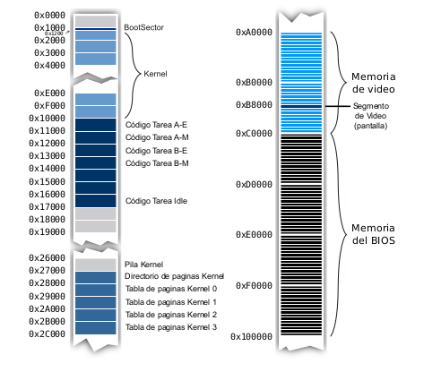
\includegraphics[width=90mm]{ej_3/img_ej_3.png}
\end{figure}

Para esto, en la función \texttt{mmu\_inicializar\_dir\_kernel}. Seteamos la direccion de la page directory en 0x27000 y de la page table 0 en 0x28000 como indica la figura.\\

Luego llamamos a \texttt{mmu\_empty\_mapping} que se encarga de inicializar las entradas 1 a 1024 de la page directory con base 0x00000 y atributos 0x00.\\
y a la función \texttt{mmu\_identity\_mapping} que se mapea con identity mapping las entradas 0 a 1024 de la page table, con atributos p=1 y r/w=1.\\
La entrada 0 de la page directory tiene como base la dirección de la page table 0 (0x28000) y atributos p=1 y r/w=1.\\

Una vez creadas estas estructuras, habilitamos la paginación cargando en cr3 la dirección del page directory (0x27000) y seteando en 1 el bit más significativo de cr0.\\

